\chapter{Publishing and Subscribing}
\label{sec:hla-pubsub}

In this chapter,
we present two Trick simulations:
one that publishes sine wave data via HLA
and one that subscribes.
Together, these represent a distributed, HLA
version of the simple publish/subscribe simulation that was discussed
in Section~\ref{sec:simplesine-pubsub-sdefine} on page~\pageref{sec:simplesine-pubsub-sdefine}.

% ------------------------------------------------------------------------
\section{{\tt SIM\_simplesine\_hla\_pub}}
This section discusses the \sdefine file for a publisher.
The file is very similar to that discussed in
Section~\ref{sec:SIM-simplesine-hla-join-sdefine}
on page~\pageref{sec:SIM-simplesine-hla-join-sdefine},
except that there is no subscriber:
the subscriber {\tt sim\_object} is gone,
the publisher no longer has a job to copy data to the subscriber, and
there is no Trick {\tt integrate} directive for the
subscriber's numerical integraion.

An abbreviated version file is shown below.
(The full {\tt THLA} and {\tt THLA\_INIT} sim objects
are identical to those in the {\tt SIM\_simplesine\_hla\_join} file.)

\begin{lstlisting}[caption={{\tt SIM\_simplesine\_hla\_pub} \sdefine},label={list:SIM-simplesine-hla-pub-sdefine}]
#include "S_properties"

#define PROPAGATE_TIMESTEP 0.25

sim_object
{
  sim_services/include: EXECUTIVE exec (sim_services/include/executive.d) ;

  (automatic) sim_services/input_processor:
    input_processor( INPUT_PROCESSOR* IP = &sys.exec.ip ) ;
} sys ;

sim_object
{
  simplesine: simplesine_T simplesine (simplesine/data/simplesine.d);

  (initialization) simplesine:
    simplesine_calc(
      simplesine_T* P = &publisher.simplesine,
      double t = sys.exec.out.time );
  (PROPAGATE_TIMESTEP, scheduled) simplesine:
    simplesine_calc(
      simplesine_T* P = &publisher.simplesine,
      double t = sys.exec.out.time );
} publisher ;

#include "S_modules/THLA.sm"

sim_object {
  ...
} THLA_INIT;
\end{lstlisting}

% ------------------------------------------------------------------------
\section{{\tt SIM\_simplesine\_hla\_sub}}
This section discusses the \sdefine file for a \TrickHLA\ publisher.
Like the publisher above, this file is similar to the \sdefine file for
the non-HLA publisher/subscriber
in Section~\ref{sec:simplesine-pubsub-sdefine} on page~\pageref{sec:simplesine-pubsub-sdefine},
except that this file has no publisher object.
An abbreviated version of the subscriber's \sdefine is shown below.

\begin{lstlisting}[caption={{\tt SIM\_simplesine\_hla\_sub} \sdefine},label={list:SIM-simplesine-hla-sub-sdefine}]
#include "S_properties"

#define PROPAGATE_TIMESTEP 0.25
#define COPY_TIMESTEP 5.0

sim_object
{
  sim_services/include: EXECUTIVE exec (sim_services/include/executive.d) ;

  (automatic) sim_services/input_processor:
    input_processor( INPUT_PROCESSOR* IP = &sys.exec.ip ) ;
} sys ;


sim_object
{
  sim_services/include: INTEGRATOR integ (simplesine/data/integ.d);
  simplesine: simplesine_T simplesine;
  simplesine: simplesine_T err;

  (initialization) simplesine:
    simplesine_calc(
      simplesine_T* P = &subscriber.simplesine,
      double t = sys.exec.out.time );

  (derivative) simplesine:
    simplesine_deriv( simplesine_T* p = &subscriber.simplesine );

  (integration) simplesine:
    simplesine_integ(
      INTEGRATOR* I = &subscriber.integ,
      simplesine_T* p = &subscriber.simplesine );

  (PROPAGATE_TIMESTEP, scheduled) simplesine:
    simplesine_calcError(
      double t = sys.exec.out.time,
      simplesine_T* s = &subscriber.simplesine,
      simplesine_state_T* err = &subscriber.err.state );

} subscriber ;

integrate (PROPAGATE_TIMESTEP) subscriber;

#include "S_modules/THLA.sm"

sim_object {
  ...
} THLA_INIT;
\end{lstlisting}

% ------------------------------------------------------------------------
\section{Publisher input file}

The publisher's input file is shown below.
It is very similar to the input file used for the join example
in the previous chapter.
The differences are
\begin{itemize}
\item{
  this federate has a different name ({\em publisher}),
}
\item{
  the simulation waits for the {\em subscriber} federate to
  join the federation, and
}
\item{
  one object class is defined to the data which this simulation
  publishes.
}
\end{itemize}

The last difference is the most significant.
To add object classes to a simulation, all that is required is that
you declare them in the input file.\footnote{
  Of course, the object class in question must already be declared in
  the FOM.
}
For this simulation,
the relevant additions to the input file are shown below.

\begin{lstlisting}[caption={{\tt SIM\_simplesine\_hla\_pub} input file},label={list:hla-pub-input}]
// This federate has one object which is publishes.
THLA.manager.obj_count = 1;
THLA.manager.objects   = alloc(THLA.manager.obj_count);

// Configure the object this federate owns and will publish.
THLA.manager.objects[0].FOM_name            = "SimplesineStateAndParameters";
THLA.manager.objects[0].name                = "simplesineStateAndParameters";
THLA.manager.objects[0].create_HLA_instance = true;
THLA.manager.objects[0].attr_count          = 6;
THLA.manager.objects[0].attributes          = alloc(THLA.manager.objects[0].attr_count);

THLA.manager.objects[0].attributes[0].FOM_name      = "Time";
THLA.manager.objects[0].attributes[0].trick_name    = "sys.exec.out.time";
THLA.manager.objects[0].attributes[0].config        = THLA_CYCLIC;
THLA.manager.objects[0].attributes[0].publish       = true;
THLA.manager.objects[0].attributes[0].locally_owned = true;
THLA.manager.objects[0].attributes[0].rti_encoding  = THLA_LITTLE_ENDIAN;

THLA.manager.objects[0].attributes[1].FOM_name      = "Value";
THLA.manager.objects[0].attributes[1].trick_name    = "publisher.simplesine.state.x";
THLA.manager.objects[0].attributes[1].config        = THLA_INITIALIZE + THLA_CYCLIC;
THLA.manager.objects[0].attributes[1].publish       = true;
THLA.manager.objects[0].attributes[1].locally_owned = true;
THLA.manager.objects[0].attributes[1].rti_encoding  = THLA_LITTLE_ENDIAN;

THLA.manager.objects[0].attributes[2].FOM_name      = "dvdt";
THLA.manager.objects[0].attributes[2].trick_name    = "publisher.simplesine.state.x_dot";
THLA.manager.objects[0].attributes[2].config        = THLA_CYCLIC;
THLA.manager.objects[0].attributes[2].publish       = true;
THLA.manager.objects[0].attributes[2].locally_owned = true;
THLA.manager.objects[0].attributes[2].rti_encoding  = THLA_LITTLE_ENDIAN;

THLA.manager.objects[0].attributes[3].FOM_name      = "Phase";
THLA.manager.objects[0].attributes[3].trick_name    = "publisher.simplesine.params.phi";
THLA.manager.objects[0].attributes[3].config        = THLA_CYCLIC;
THLA.manager.objects[0].attributes[3].publish       = true;
THLA.manager.objects[0].attributes[3].locally_owned = true;
THLA.manager.objects[0].attributes[3].rti_encoding  = THLA_LITTLE_ENDIAN;

THLA.manager.objects[0].attributes[4].FOM_name      = "Frequency";
THLA.manager.objects[0].attributes[4].trick_name    = "publisher.simplesine.params.w";
THLA.manager.objects[0].attributes[4].config        = THLA_CYCLIC;
THLA.manager.objects[0].attributes[4].publish       = true;
THLA.manager.objects[0].attributes[4].locally_owned = true;
THLA.manager.objects[0].attributes[4].rti_encoding  = THLA_LITTLE_ENDIAN;

THLA.manager.objects[0].attributes[5].FOM_name      = "Amplitude";
THLA.manager.objects[0].attributes[5].trick_name    = "publisher.simplesine.params.A";
THLA.manager.objects[0].attributes[5].config        = THLA_CYCLIC;
THLA.manager.objects[0].attributes[5].publish       = true;
THLA.manager.objects[0].attributes[5].locally_owned = true;
THLA.manager.objects[0].attributes[5].rti_encoding  = THLA_LITTLE_ENDIAN;
\end{lstlisting}

This set of inputs tells \TrickHLA\ that the simulation will be publishing
an object with six attributes.

Lines 2-3 indicate that only a single object is involved.

Lines 6-7 specify that the object instance will be named
{\tt simplesineStateAndParameters} and that it is an instance of the class
{\tt SimplesineStateAndParameters} (which must be defined in the FOM).

Line 8 indicates that the instance will be owned by this simulation.

Lines 10-11 specify that the simulation is interested in six attributes
of the instance -- in this case all of them.

The subsequent lines specify per-attribute settings:
the name of the attribute as specified in the class definition in the FOM,
the name of the Trick variable associated with the attribute,
whether the attribute is owned locally,
whether this simulation intends to publish values for the attribute,
and how the data is to be encoded when it is sent over the network.
Notice that the trick variables specified are {\simplesine} parameters
and state located in the publisher object.

By associating Trick variables with attributes in this fashion,
whenever the \TrickHLA\ infrastructure sends out updates
(as defined in the {\tt THLA} object in the \sdefine file),
the current value of the corresponding Trick variable will be used.
Simulation developers need do nothing explicit to send data --
the \TrickHLA\ infrastructure handles that task.

% ------------------------------------------------------------------------
\section{Subscriber input file}

Like the publisher, the subscriber's input file is similar to the join example
in the previous chapter.
The differences are
\begin{itemize}
\item{
  this federate has a different name ({\em subscriber}).
}
\item{
  the simulation waits for the {\em publisher} federate to join
  the federation, and
}
\item{
  an object class is defined for the data to which this federate
  subscribes.
}
\end{itemize}

Indeed, the subscriber inputs are very similar to the publisher inputs above
with the exception that
local ownership is turned off,
publishing is turned off, and
subscribing is turned on.

The relevant object declarations are shown below.

\begin{lstlisting}[caption={{\tt SIM\_simplesine\_hla\_sub} input file},label={list:hla-sub-input}]
// This federate has only one object, and it subscribes to it.
THLA.manager.obj_count = 1;
THLA.manager.objects   = alloc(THLA.manager.obj_count);

// objects subscribed to
THLA.manager.objects[0].FOM_name            = "SimplesineStateAndParameters";
THLA.manager.objects[0].name                = "simplesineStateAndParameters";
THLA.manager.objects[0].create_HLA_instance = false;
THLA.manager.objects[0].attr_count          = 6;
THLA.manager.objects[0].attributes          = alloc(THLA.manager.objects[0].attr_count);

THLA.manager.objects[0].attributes[0].FOM_name      = "Time";
THLA.manager.objects[0].attributes[0].trick_name    = "sys.exec.out.time";
THLA.manager.objects[0].attributes[0].config        = THLA_CYCLIC;
THLA.manager.objects[0].attributes[0].publish       = false;
THLA.manager.objects[0].attributes[0].subscribe     = true;
THLA.manager.objects[0].attributes[0].locally_owned = false;
THLA.manager.objects[0].attributes[0].rti_encoding  = THLA_LITTLE_ENDIAN;

THLA.manager.objects[0].attributes[1].FOM_name      = "Value";
THLA.manager.objects[0].attributes[1].trick_name    = "subscriber.simplesine.state.x";
THLA.manager.objects[0].attributes[1].config        = THLA_INITIALIZE + THLA_CYCLIC;
THLA.manager.objects[0].attributes[1].publish       = false;
THLA.manager.objects[0].attributes[1].subscribe     = true;
THLA.manager.objects[0].attributes[1].locally_owned = false;
THLA.manager.objects[0].attributes[1].rti_encoding  = THLA_LITTLE_ENDIAN;

THLA.manager.objects[0].attributes[2].FOM_name      = "dvdt";
THLA.manager.objects[0].attributes[2].trick_name    = "subscriber.simplesine.state.x_dot";
THLA.manager.objects[0].attributes[2].config        = THLA_CYCLIC;
THLA.manager.objects[0].attributes[2].publish       = false;
THLA.manager.objects[0].attributes[2].subscribe     = true;
THLA.manager.objects[0].attributes[2].locally_owned = false;
THLA.manager.objects[0].attributes[2].rti_encoding  = THLA_LITTLE_ENDIAN;

THLA.manager.objects[0].attributes[3].FOM_name      = "Phase";
THLA.manager.objects[0].attributes[3].trick_name    = "subscriber.simplesine.params.phi";
THLA.manager.objects[0].attributes[3].config        = THLA_CYCLIC;
THLA.manager.objects[0].attributes[3].publish       = false;
THLA.manager.objects[0].attributes[3].subscribe     = true;
THLA.manager.objects[0].attributes[3].locally_owned = false;
THLA.manager.objects[0].attributes[3].rti_encoding  = THLA_LITTLE_ENDIAN;

THLA.manager.objects[0].attributes[4].FOM_name      = "Frequency";
THLA.manager.objects[0].attributes[4].trick_name    = "subscriber.simplesine.params.w";
THLA.manager.objects[0].attributes[4].config        = THLA_CYCLIC;
THLA.manager.objects[0].attributes[4].publish       = false;
THLA.manager.objects[0].attributes[4].subscribe     = true;
THLA.manager.objects[0].attributes[4].locally_owned = false;
THLA.manager.objects[0].attributes[4].rti_encoding  = THLA_LITTLE_ENDIAN;

THLA.manager.objects[0].attributes[5].FOM_name      = "Amplitude";
THLA.manager.objects[0].attributes[5].trick_name    = "subscriber.simplesine.params.A";
THLA.manager.objects[0].attributes[5].config        = THLA_CYCLIC;
THLA.manager.objects[0].attributes[5].publish       = false;
THLA.manager.objects[0].attributes[5].subscribe     = true;
THLA.manager.objects[0].attributes[5].locally_owned = false;
THLA.manager.objects[0].attributes[5].rti_encoding  = THLA_LITTLE_ENDIAN;
\end{lstlisting}


\section{Output}

Together, these two simulations do in a distributed fashion what
the single simulation did in Chapter~\ref{sec:simplesine-sim}.
The publisher generates sine wave data and periodically sends updates
to the subscriber.
The subscriber receives the periodic updates and extrapolates the state
until the next update arrives.

Figure~\ref{fig:hla-pub-output} shows the sine wave as generated on
the publisher.
Figure~\ref{fig:hla-sub-noInteg-output} shows the sine wave as received by
the subscriber with numerical integration disabled to emphasize the
time of arrival of the data.
Figure~\ref{fig:hla-sub-output} shows the sine wave generated by the
subscriber based on data received from the publisher with subscriber-side
numerical integration between updates.

Close inspection of the publisher and subscriber plots reveals that
they are slightly out of phase, hence the relatively large error
in the third plot.
This phase lag is due to HLA time management {\em lookahead},
which is 1.0sec in this case.
Indeed, this effect can be seen clearly at $t=1$, since up until that
point the subscriber was integrating based solely on initial conditions
(not based on any data received from the publisher),
but at $t=1$, the first data arrives from the publisher but it is
approximately 1sec late, resulting in a discontinuity in the data.
This lookahead-induced effect can be compensated using \TrickHLA\ features
discussed in Chapter~\ref{sec:hla-lag}.

\begin{figure}[b]
  \begin{center}
    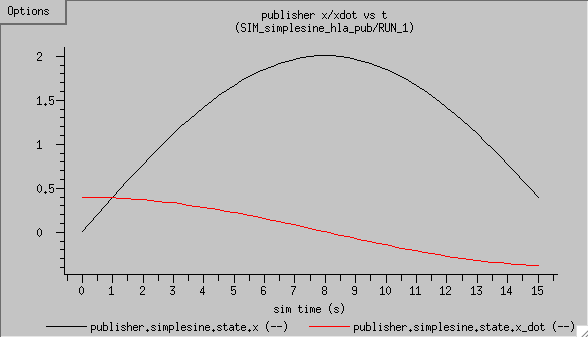
\includegraphics[width=4.5in]{TrickHLAUser-SIM-hla-pub.png}
  \end{center}
\caption{Output from {\tt SIM\_simplesine\_hla\_pub}}
\label{fig:hla-pub-output}
\end{figure}

\begin{figure}[b]
  \begin{center}
    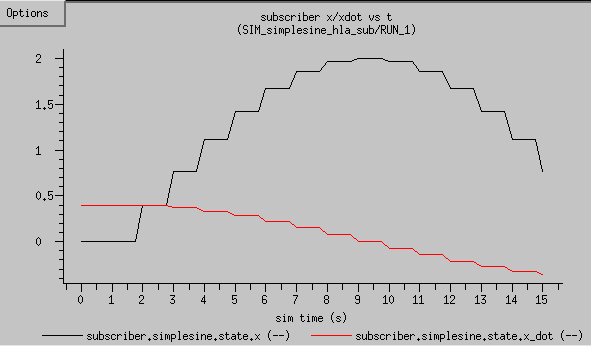
\includegraphics[width=4.5in]{TrickHLAUser-SIM-hla-sub-noInteg.png}
  \end{center}
\caption{Output from {\tt SIM\_simplesine\_hla\_sub} (no integration)}
\label{fig:hla-sub-noInteg-output}
\end{figure}

\begin{figure}[b]
  \begin{center}
    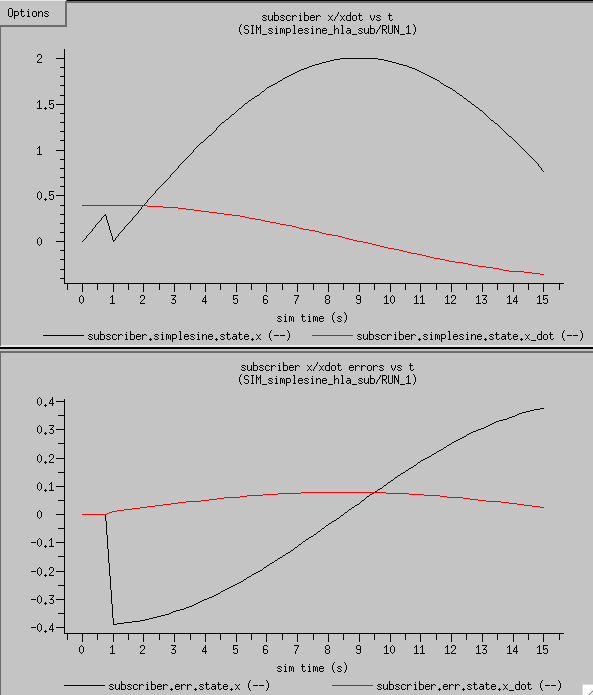
\includegraphics[width=4.5in]{TrickHLAUser-SIM-hla-sub.png}
  \end{center}
\caption{Output from {\tt SIM\_simplesine\_hla\_pub}}
\label{fig:hla-sub-output}
\end{figure}


